\section{Introduction}
This document shows how to use the survival records script for setting up automatically updated survival records that are displayed on Google Spreadsheets.
\paragraph{Small note}
I am going to try to update this document with a lot of screenshots to make it an easy step-by-step tutorial. However, the spreasheet is constantly being changed so the actual document may end up looking different.
\subsection{Purpose}
Why should we bother with keeping track of survival records anyway? This project is not as serious as it seems and mostly serves as a sideproject of mine. It serves as a way for me to learn Python and to practice a little bit of programming. Other than that, the records are not meant to be taken very seriously. However, it is good to keep track of and recognize achievements made by our community of survival players.

There are many people playing survival mode in Left 4 Dead 1 and Left 4 Dead 2 from all over the world, and it is a good opportunity to make new online friends and collaborate with them towards a common goal. The Left 4 Dead series are known to be high quality cooperative games that stress teamwork, and the addition of goals and records makes the game refreshing and endlessly replayable for many survival enthusiasts.

\subsection{How it works}
After each game of survival, the game displays the statistics of the round that you just played. This includes the duration of the round and the number of common infected, special infected and tanks killed. The numbers will typed by someone (maybe you!) onto a Google Spreadsheet for the purpose of keeping track of records. Once the numbers are input onto the spreadsheet, the spreadsheet maintainer runs the provided Python script in order to update the spreadsheet. The best time, kills, and other statistics are calculated and displayed on the updated spreadsheet. In the next sections, the software behind the recording system will be explained.

\subsubsection{Google Spreadsheets}
Google spreadsheets is part of the Google Docs office suite, which is an online service designed to allow users to collaborate on office documents. The spreadsheets are a collection of tables, and consist of multiple pages called worksheets. \figurename\ \ref{fig:sample1} shows what a Google Spreadsheet looks like in a web browser.
\begin{figure}[htb!]
\centering
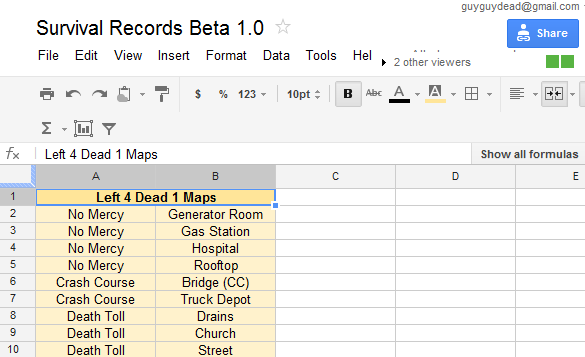
\includegraphics[width=0.40\columnwidth]{sample_screen_1}
\caption{Google Spreadsheet Opened in Web Browser}
\label{fig:sample1}
\end{figure}

One of the interesting features of Google Docs is that any changes made to the web documents are instantly updated and seen by people on the Internet. In this way, we can imagine having a document that outputs real-time statistics, in our case, of the game Left 4 Dead.

\subsubsection{Google Data API}
As well as being able to edit spreadsheets from a web browser, Google has provided a way to communicate to their servers and automatically update Google Spreadsheets: the Google Data API (Application Programming Interface). What this means is that anyone can download the provided programming library and use it to read from and write to a Google Spreadsheet by writing a simple program.

\subsubsection{Python}
Python is a relatively new programming language suitable for scripting. I chose Python because it is an interesting language that I wanted to learn through this project. \figurename\ \ref{fig:sample2} shows the output of a sample run of the Python script to update the Google Spreadsheet.
\begin{figure}[htb!]
\centering
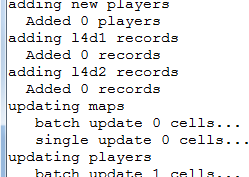
\includegraphics[width=0.30\columnwidth]{sample_screen_2}
\caption{Python Script Updating the Spreadsheet}
\label{fig:sample2}
\end{figure}
